% Created 2017-05-02 mar 16:49
\documentclass[a4paper]{scrartcl}
\usepackage[utf8]{inputenc}
\usepackage[T1]{fontenc}
\usepackage{fixltx2e}
\usepackage{graphicx}
\usepackage{longtable}
\usepackage{float}
\usepackage{wrapfig}
\usepackage{rotating}
\usepackage[normalem]{ulem}
\usepackage{amsmath}
\usepackage{textcomp}
\usepackage{marvosym}
\usepackage{wasysym}
\usepackage{amssymb}
\usepackage{hyperref}
\tolerance=1000
\usepackage{khpreamble}
\newcommand{\tustin}{\frac{2}{h}\frac{z-1}{z+1}}
\author{Kjartan Halvorsen}
\date{2016-05-06}
\title{Computerized control - final exam (30\%)}
\hypersetup{
  pdfkeywords={},
  pdfsubject={},
  pdfcreator={Emacs 24.5.1 (Org mode 8.2.10)}}
\begin{document}

\maketitle

\section*{Problem 1 (30p)}
\label{sec-1}
The definition of \emph{anaesthesia} (or unconsciousness) is being in a state in which the body does not sense pain or other stimulii. The level, or depth, of anaesthesia is usually controlled by administrating drugs to the air inhaled by the patient undergoing surgery. The \emph{Mean Arterial Pressure (MAP)} is an important indicator for how deep the anaesthesia is. Consider a system for automatized delivery of anaesthetics:
\begin{center}
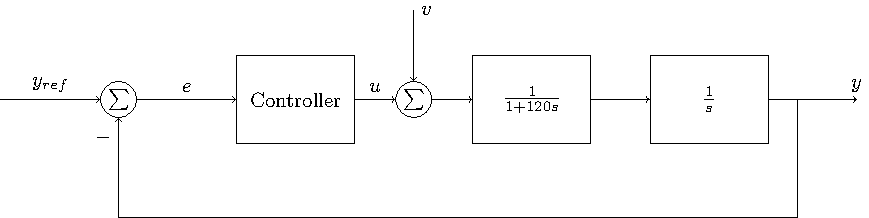
\includegraphics[width=0.999\linewidth]{anaesthesia}
\end{center}
The controller sets the position of a valve that controls the flow $u$ of anaesthetics, based on the difference between the reference MAP, $y_{ref}$, and the measured MAP, $y$.  The effect of the inflow of drug on the rate of change in the MAP of the patient is identified experimentally, and is described by the transfer function 
\[ G(s) = \frac{1}{1+120s}, \] where the time unit is seconds. The surgery involves an uncontrolled stimulus on the system, and is represented by the additive disturbance signal $v$.


\subsection*{(a) (10p)}
\label{sec-1-1}
In the figure below, plot the continuous-time poles of the patient model (plant, including integrator) on the left complex plane. Choose a reasonable sampling time $h$, and plot the discrete-time poles obtained with zero-order-hold sampling in the right complex plane. 

\begin{center}
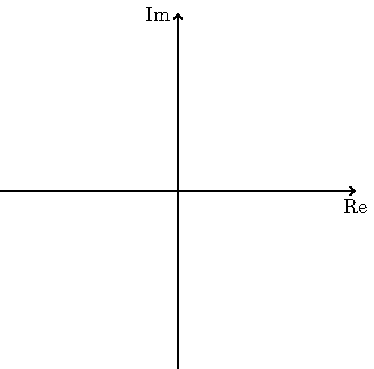
\includegraphics[width=0.4\linewidth]{imaginary-plane-empty-cartesian}
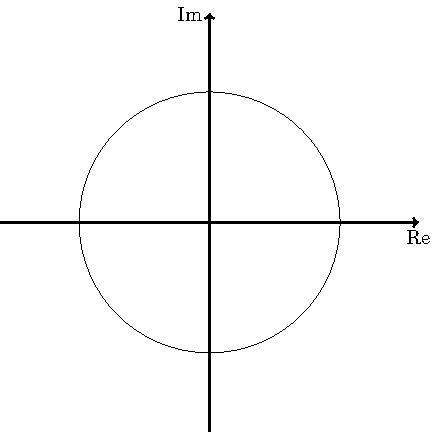
\includegraphics[width=0.4\linewidth]{imaginary-plane-empty}
\end{center}
\subsection*{(b) (20p)}
\label{sec-1-2}
A continuous-time controller for the system has been designed and is given by 
\[ F(s) = \frac{25.6(16s+1)}{100s+1}. \]

Discretize the controller using the backward difference approximation
\[ \operatorname{p} \approx \frac{\operatorname{q}-1}{\operatorname{q}h}. \]

\section*{Problem 2 (30p)}
\label{sec-2}
An alternative, discrete-time version of the patient-model in Problem 1 is given by
\[ H(z) = \frac{0.6z + 0.5}{z(z^2 - 1.9z + 0.9)}. \]
Apart from being discrete, this model differs from the one in Problem 1 by also including a time-delay.  The system is to be controlled using an RST-controller as in the figure below.
\begin{center}
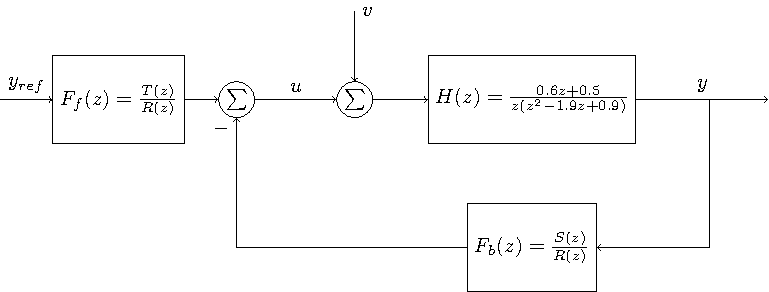
\includegraphics[width=\linewidth]{rst-block}
\end{center}

Choose the correct answer to each question below. \textbf{Motivate your answers briefly with 1-2 sentences.}

\subsection*{(a) (15p)}
\label{sec-2-1}
Which of the following pulse-transfer functions describes the closed-loop response of the system to the disturbance $v$, i.e. the pulse-transfer function from $v$ to $y$?  
\begin{enumerate}
\item \( \frac{R(z) \left(0.6 z + 0.5\right)}{S(z) z \left(z^{2} - 1.9 z + 0.9\right) + R(z) \left(0.6 z + 0.5\right)} \)
\item \(\frac{S(z) \left(0.6 z + 0.5\right)}{R(z) z \left(z^{2} - 1.9 z + 0.9\right) + S(z) \left(0.6 z + 0.5\right)}\)
\item \( \frac{R(z) \left(0.6 z + 0.5\right)}{R(z) z \left(z^{2} - 1.9 z + 0.9\right) + S(z) \left(0.6 z + 0.5\right)} \)
\end{enumerate}
\subsection*{(b) (15p)}
\label{sec-2-2}
Assume that the desired closed-loop characteristic polynomial is
\[ A_{cl}(z) = (z^2 - 1.4z + 0.5)(z-0.6)(z-0.5)^2. \]

Which of the following pairs of $S(z)$ and $R(z)$ controller polynomials is appropriate in order to determine the controller parameters from the Diophantine equation?
\begin{enumerate}
\item \(R(z) = z + r_1, \quad S(z) = s_0z + s_1 \)
\item \(R(z) = z^2 + r_1z + r_2, \quad S(z) = s_1z + s_2 \)
\item \(R(z) = z^2 + r_1z + r_2, \quad S(z) = s_0z^2 + s_1z + s_2 \)
\item \(R(z) = z + r_1, \quad S(z) = s_1 \)
\end{enumerate}


\section*{Problem 3 (40p)}
\label{sec-3}
Consider the discrete-time state-space model
 \begin{equation*}
 \begin{split}
  x(k+1) &= \bbm 0.9 & 0\\0 & 1\ebm x(k) + \bbm 1\\1 \ebm u(k)\\
  y(k) &= \bbm -10.4 & 11.0 \ebm.
 \end{split}
\end{equation*}

\subsection*{(a) (10p)}
\label{sec-3-1}
What are the poles of the system? Is the system stable?

\subsection*{(b) (10p)}
\label{sec-3-2}
Show that the state-space model corresponds to the pulse-transfer function
\[ H(z) = -\frac{10.4}{z-0.9} + \frac{11.0}{z-1} = \frac{0.6z + 0.5}{z^2 - 1.9z + 0.9}. \]
\subsection*{(b) (20p)}
\label{sec-3-3}
We want to determine a linear state feedback $u(k) = -Lx(k) + u_c(k)$ such that the closed-loop system has poles in \[ 0.6 \pm i0.3 \] Describe in a few steps and 5-8 sentences, the procedure to determine the controller parameters in $L$. You do \textbf{not} need to do the calculations or solve the equations. 


\section*{Solutions}
\label{sec-4}
\subsection*{Problem 1}
\label{sec-4-1}
\subsubsection*{(a)}
\label{sec-4-1-1}
The first-order system describing the response to the flow of drug has time constant $T=\unit{120}{\second}$, which corresponds to a rising time $T_r=2.2T$. The appropriate rule-of-thumb says 4-10 sampling periods per rise time, which gives
\[ h \approx \unit{26.4}{\second} - \unit{66.0}{\second}. \]
Choosing, for instance $h=40.0$ gives one discrete-time pole in \(0.717\) and one in \(1\).  
\begin{center}
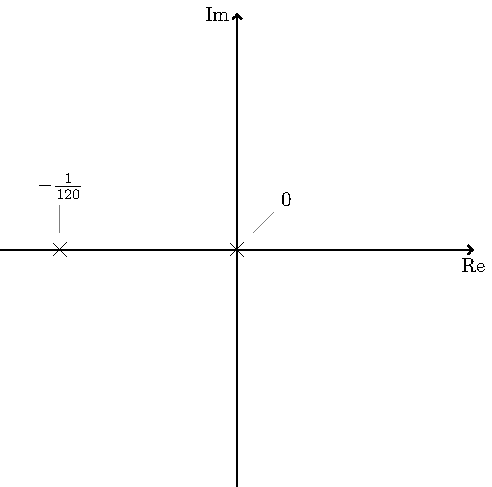
\includegraphics[width=0.4\linewidth]{imaginary-plane-ct-poles-final}
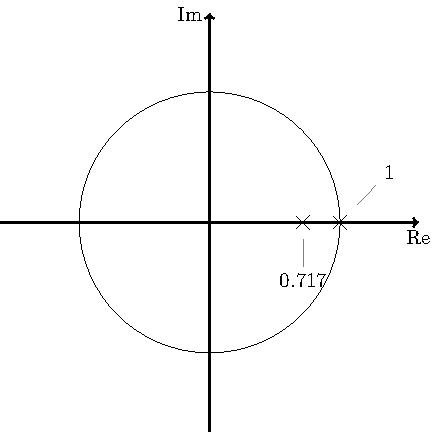
\includegraphics[width=0.4\linewidth]{imaginary-plane-dt-poles-final}
\end{center}
\subsubsection*{(b)}
\label{sec-4-1-2}
Inserting \[s = \frac{z-1}{zh}\] into the expression for the controller gives
\[ H(z) = F(s)|_{s=\frac{z-1}{zh}} = 25.6\frac{(16+h)z -16}{(100+h)z - 100}. \]

\subsection*{Problem 2}
\label{sec-4-2}
\subsubsection*{(a)}
\label{sec-4-2-1}
The correct answer is \textbf{3}. \(\frac{R(z) \left(0.6 z + 0.5\right)}{R(z) z \left(z^{2} - 1.9 z + 0.9\right) + S(z) \left(0.6 z + 0.5\right)}\). This can be found by calculation in the block-diagram. with $H(z) = \frac{B}{A}$, the pulse-transfer function from $v$ to $y$ is
\[ H_v(z) = \frac{\frac{B}{A}}{1 + \frac{B}{A}\frac{S}{R}} = \frac{R(z)B(z)}{A(z)R(z) + B(z)S(z)}. \]
We see that alternative 1 and 3 has the correct numerator. But only alternative 3 has also the correct denominator.

\subsubsection*{(b)}
\label{sec-4-2-2}
The correct answer is \textbf{3}.  \(R(z) = z^2 + r_1z + r_2, \quad S(z) = s_0z^2 + s_1z + s_2 \). The desired closed-loop characteristic polynomial has order 5. On the left-hand side of the Diophantine equation 
\[ R(z) z \left(z^{2} - 1.9 z + 0.9\right) + S(z) \left(0.6 z + 0.5\right) = A_{cl}(z) \]
we see that $A(z)$ has order 3. Then $R(z)$ should have order two and $S(z)$ likewise, since this gives five unknown controller parameters to be solved from the five equations that the fifth-order Diophantine equation gives. 

\subsection*{Problem 3}
\label{sec-4-3}
\subsubsection*{(a)}
\label{sec-4-3-1}
The poles are the eigenvalues of the $\Phi$ matrix. Here the matrix is diagonal, so the eigenvalues are simply the diagonal elements $0.9$ and $1$. For stability, the poles should be strict \emph{inside} the unit circle. There is a pole in 1, corresponding to an integrator, so this system is \textbf{not stable}.

\subsubsection*{(b)}
\label{sec-4-3-2}
The pulse-transfer function is found by calculating
\begin{equation*}
  \begin{split}
 H(z) &= C \left( zI - \Phi\right)^{-1} \Gamma\\
      &= C \bbm z-0.9 & 0\\0 & z-1 \ebm ^{-1} \Gamma \\
      &= C \bbm \frac{1}{z-0.9} & 0\\ 0 & \frac{1}{z-1} \ebm \Gamma \\
      &= \bbm -10.4 & 11.0 \ebm \bbm \frac{1}{z-0.9} & 0\\ 0 & \frac{1}{z-1} \ebm \bbm 1\\1\ebm \\
      &= - \frac{10.4}{z-0.9} + \frac{11.0}{z-1}.
  \end{split}
 \end{equation*}


\subsubsection*{(c)}
\label{sec-4-3-3}
The procedure is as follows. 
\begin{enumerate}
\item From the desired closed-loop poles, we calculate the desired close-loop characteristic polynomial
\[ A_{cl}(z) = (z-p_1)(z - p_2) = (z-0.6+0.3i)(z-0.6-0.3i) = z^2 -1.2z + 0.45.\]
\item With the linear state feedback we get the closed-loop system on state space form
\begin{equation*}
 \begin{split}
 x(k+1) &= \left(\Phi - \Gamma L\right)x(k) + \Gamma u_c(k)\\
 y(k) &= C x(k).
 \end{split}
\end{equation*}
The characteristic polynomial is given by
\[ \det \left(zI - (\Phi - \Gamma L)\right), \]
which is a polynomial of degree 2 in this case.
\item Set this polynomial equal to the desired polynomial
\[ \det \left(zI - (\Phi - \Gamma L)\right) = z^2 - 1.2z + 0.45. \]
Form a linear system of equations in the elements of $L$ by setting each coefficient equal. This gives 2 equations in the two unknowns $l_1$ and $l_2$.
\end{enumerate}
% Emacs 24.5.1 (Org mode 8.2.10)
\end{document}